\chapter{Interest Rate Swaps and Swaptions}\label{interest-rate-swaps-and-swaptions}

In the previous Chapters we have already introduces a particular type of swap, the Overnight Index Swap, here we will introduce a more general Interest Rate Swap and see how it can underlying a Swaption, the analogous of the European options for interest rate market.

\subsection{Interest Rate Swaps}\label{interest-rate-swaps}

Interest rate swaps (IRS) consist of two legs a floating and a fixed. The
contract parameters are:

\begin{itemize}
\tightlist
\item
  start date \(d_0\);
\item
  notional \(N\);
\item
  fixed rate \(K\);
\item
  floating rate tenor (months);
\item
  maturity (years).
\end{itemize}

The floating leg pays the reference LIBOR fixing at a frequency equal to
the tenor of the floating rate, so for example an IRS on a 3-month
LIBOR will pay a floating coupon every three months, an IRS on 6-month
EURIBOR pays the floating coupon every six months and so on.

The fixed leg pays a predetermined cash flow at annual frequency,
regardless of the tenor of the underlying floating rate. 

For simplicity we will only consider swaps with maturities which are multiples of 1
year.

Before going into the details of the valuation of IRSs, we need to
modify the \texttt{generate\_swap\_dates} function in our
\texttt{finmarkets} module to generate the payment dates for both the
fixed and floating legs. The modification consists of the addition of a new input
parameter, the tenor, which was previously set to 12 months.

\begin{tcolorbox}[breakable, size=fbox, boxrule=1pt, pad at break*=1mm,colback=cellbackground, colframe=cellborder]
\begin{Verbatim}[commandchars=\\\{\}]
\PY{k+kn}{from} \PY{n+nn}{datetime} \PY{k}{import} \PY{n}{date}
\PY{k+kn}{from} \PY{n+nn}{dateutil}\PY{n+nn}{.}\PY{n+nn}{relativedelta} \PY{k}{import} \PY{n}{relativedelta}
    
\PY{k}{def} \PY{n+nf}{generate\PYZus{}swap\PYZus{}dates}\PY{p}{(}\PY{n}{start\PYZus{}date}\PY{p}{,} \PY{n}{n\PYZus{}months}\PY{p}{,} \PY{n}{tenor\PYZus{}months}\PY{o}{=}\PY{l+m+mi}{12}\PY{p}{)}\PY{p}{:}
    \PY{n}{dates} \PY{o}{=} \PY{p}{[}\PY{p}{]}
    \PY{k}{for} \PY{n}{n} \PY{o+ow}{in} \PY{n+nb}{range}\PY{p}{(}\PY{l+m+mi}{0}\PY{p}{,} \PY{n}{n\PYZus{}months}\PY{p}{,} \PY{n}{tenor\PYZus{}months}\PY{p}{)}\PY{p}{:}
        \PY{n}{dates}\PY{o}{.}\PY{n}{append}\PY{p}{(}\PY{n}{start\PYZus{}date} \PY{o}{+} \PY{n}{relativedelta}\PY{p}{(}\PY{n}{months}\PY{o}{=}\PY{n}{n}\PY{p}{)}\PY{p}{)}
    \PY{n}{dates}\PY{o}{.}\PY{n}{append}\PY{p}{(}\PY{n}{start\PYZus{}date} \PY{o}{+} \PY{n}{relativedelta}\PY{p}{(}\PY{n}{months}\PY{o}{=}\PY{n}{n\PYZus{}months}\PY{p}{)}\PY{p}{)}
    \PY{k}{return} \PY{n}{dates}

\PY{n}{generate\PYZus{}swap\PYZus{}dates}\PY{p}{(}\PY{n}{date}\PY{o}{.}\PY{n}{today}\PY{p}{(}\PY{p}{)}\PY{p}{,} \PY{l+m+mi}{16}\PY{p}{,} \PY{l+m+mi}{3}\PY{p}{)}

[datetime.date(2020, 10, 15),
 datetime.date(2021, 1, 15),
 datetime.date(2021, 4, 15),
 datetime.date(2021, 7, 15),
 datetime.date(2021, 10, 15),
 datetime.date(2022, 1, 15),
 datetime.date(2022, 2, 15)]
\end{Verbatim}
\end{tcolorbox}
        
Using this function and the contract parameters we will be able to
determine a sequence of payment dates for each leg of the IRS.

\subsection{IRS Valuation}\label{irs-valuation}

Let \(d_0=d_0^{\mathrm{fixed}},...,d_p^{\mathrm{fixed}}\) be the fixed
leg payment dates and
\(d_0=d_0^{\mathrm{float}},...,d_p^{\mathrm{float}}\) be the floating
leg payment dates, and let's use the following notation:

\begin{itemize}
\tightlist
\item
  \(d\) the pricing date;
\item
  \(D(d, d')\) the discount factor observed in date \(d\) for the value
  date \(d'\);
\item
  \(F(d, d', d'')\) the forward rate observed in date \(d\) for the
  period \([d', d'']\). The rate tenor is \(\tau = d'' - d'\).
\end{itemize}

The NPV of the fixed leg is calculated as follows:

\[\mathrm{NPV}_{\mathrm{fixed}}(d, K) = N\cdot K\cdot\sum_{i=1}^{n}D(d, d_{i}^{\mathrm{fixed}})\]
while the NPV of the floating leg is calculated as follows:

\[\mathrm{NPV}_{\mathrm{float}}(d) = N\cdot\sum_{i=1}^{m}F(d, d_{j-1}^{\mathrm{float}}, d_{j}^{\mathrm{float}}) \cdot \frac{d_{j}^{\mathrm{float}}-d_{j-1}^{\mathrm{float}}}{360}
\cdot D(d, d_{i}^{\mathrm{float}})\]

Therefore the NPV of the swap (seen from the point of view of the
counter-party which receives the floating leg) is

\[\mathrm{NPV}(d, K) = \mathrm{NPV}_{\mathrm{float}}(d) - \mathrm{NPV}_{\mathrm{fixed}}(d, K)\]

For reasons which will become apparent later, it's actually more
convenient to express the NPV of an IRS as a function of the fair value
fixed rate \(S\) of the IRS, also known as the \textbf{swap rate}. \(S\)
is the value of K which makes \(\mathrm{NPV}(d)=0\).

On the basis of the previous expressions, we can easily calculate \(S\)
as:

\[\mathrm{NPV}_{\mathrm{fixed}}(d, S) = \mathrm{NPV}_{\mathrm{float}}(d)\]
\[N\cdot S\cdot\sum_{i=1}^{n}D(d, d_{i}^{\mathrm{fixed}}) = N\cdot\sum_{i=1}^{m}F(d, d_{j-1}^{\mathrm{float}}, d_{j}^{\mathrm{float}}) \cdot \frac{d_{j}^{\mathrm{float}}-d_{j-1}^{\mathrm{float}}}{360} \cdot D(d, d_{i}^{\mathrm{float}})\]
\[S=\frac{\sum_{i=1}^{m}F(d, d_{j-1}^{\mathrm{float}}, d_{j}^{\mathrm{float}}) \cdot \frac{d_{j}^{\mathrm{float}}-d_{j-1}^{\mathrm{float}}}{360}
\cdot D(d, d_{i}^{\mathrm{float}})}{\sum_{i=1}^{n}D(d, d_i^{\mathrm{fixed}})} \]

Once we have calculated \(S\), we can express the \(\mathrm{NPV}\) of an
IRS as follows:

\begin{align*}&\mathrm{NPV}(d, K) = \mathrm{NPV}_{\mathrm{float}}(d) - \mathrm{NPV}_{\mathrm{fixed}}(d, K) = & \\ \\ &= \underbrace{\mathrm{NPV}_{\mathrm{float}}(d) - \mathrm{NPV}_{\mathrm{fixed}}(d, S)}_{\mathrm{=\;0}} + \mathrm{NPV}_{\mathrm{fixed}}(d, S) - \mathrm{NPV}_{\mathrm{fixed}}(d, K) & \\ & = N\cdot(S-K)\cdot\underbrace{\sum_{i=1}^{n}D(d, d_{i}^{\mathrm{fixed}})}_{\mathrm{'annuity'}}
\end{align*}

For convenience the relevant inputs that will be used later (LIBOR and discount curve definitions) have been saved in the files \href{https://drive.google.com/file/d/1dm5oZnZKmJM6UrV0L32OcqD5Tzs9SI9A/view?usp=sharing}{libor\_curve.xlsx} and \href{https://drive.google.com/file/d/14R22r7m-6VpQ_P79D3qHdK0QN_mOQ_UB/view?usp=sharing}{discount\_curve.xlsx} respectively.

\begin{tcolorbox}[breakable, size=fbox, boxrule=1pt, pad at break*=1mm,colback=cellbackground, colframe=cellborder]
\begin{Verbatim}[commandchars=\\\{\}]
\PY{k+kn}{import} \PY{n+nn}{pandas} \PY{k}{as} \PY{n+nn}{pd}
\PY{k+kn}{from} \PY{n+nn}{datetime} \PY{k}{import} \PY{n}{date}
\PY{k+kn}{from} \PY{n+nn}{finmarkets} \PY{k}{import} \PY{n}{DiscountCurve}\PY{p}{,} \PY{n}{ForwardRateCurve}

\PY{n}{observation\PYZus{}date} \PY{o}{=} \PY{n}{date.today()}
\PY{n}{discount\PYZus{}data} \PY{o}{=} \PY{n}{pd}\PY{o}{.}\PY{n}{read\PYZus{}excel}\PY{p}{(}\PY{l+s+s1}{\PYZsq{}}\PY{l+s+s1}{discount\PYZus{}curve.xlsx}\PY{l+s+s1}{\PYZsq{}}\PY{p}{)}
\PY{n}{libor\PYZus{}data} \PY{o}{=} \PY{n}{pd}\PY{o}{.}\PY{n}{read\PYZus{}excel}\PY{p}{(}\PY{l+s+s1}{\PYZsq{}}\PY{l+s+s1}{libor.xlsx}\PY{l+s+s1}{\PYZsq{}}\PY{p}{)}

\PY{n}{dc} \PY{o}{=} \PY{n}{DiscountCurve}\PY{p}{(}\PY{n}{pricing\PYZus{}date}\PY{p}{,} 
                   \PY{n}{discount\PYZus{}data}\PY{p}{[}\PY{l+s+s1}{\PYZsq{}}\PY{l+s+s1}{pillar}\PY{l+s+s1}{\PYZsq{}}\PY{p}{]}\PY{o}{.}\PY{n}{dt}\PY{o}{.}\PY{n}{date}\PY{o}{.}\PY{n}{tolist}\PY{p}{(}\PY{p}{)}\PY{p}{,}
                   \PY{n}{discount\PYZus{}data}\PY{p}{[}\PY{l+s+s1}{\PYZsq{}}\PY{l+s+s1}{discount\PYZus{}factor}\PY{l+s+s1}{\PYZsq{}}\PY{p}{]}\PY{o}{.}\PY{n}{tolist}\PY{p}{(}\PY{p}{)}\PY{p}{)}

\PY{n}{fr} \PY{o}{=} \PY{n}{ForwardRateCurve}\PY{p}{(}\PY{n}{libor\PYZus{}data}\PY{p}{[}\PY{l+s+s1}{\PYZsq{}}\PY{l+s+s1}{date}\PY{l+s+s1}{\PYZsq{}}\PY{p}{]}\PY{o}{.}\PY{n}{dt}\PY{o}{.}\PY{n}{date}\PY{o}{.}\PY{n}{tolist}\PY{p}{(}\PY{p}{)}\PY{p}{,}
                      \PY{n}{libor\PYZus{}data}\PY{p}{[}\PY{l+s+s1}{\PYZsq{}}\PY{l+s+s1}{rate}\PY{l+s+s1}{\PYZsq{}}\PY{p}{]}\PY{o}{.}\PY{n}{tolist}\PY{p}{(}\PY{p}{)}\PY{p}{)}

\PY{n+nb}{print}\PY{p}{(}\PY{n}{dc}\PY{o}{.}\PY{n}{df}\PY{p}{(}\PY{n}{date}\PY{p}{(}\PY{l+m+mi}{2021}\PY{p}{,} \PY{l+m+mi}{1}\PY{p}{,} \PY{l+m+mi}{1}\PY{p}{)}\PY{p}{)}\PY{p}{)}
\PY{n+nb}{print} \PY{p}{(}\PY{n}{fr}\PY{o}{.}\PY{n}{forward\PYZus{}rate}\PY{p}{(}\PY{n}{date}\PY{p}{(}\PY{l+m+mi}{2021}\PY{p}{,} \PY{l+m+mi}{1}\PY{p}{,} \PY{l+m+mi}{1}\PY{p}{)}\PY{p}{)}\PY{p}{)}

1.0041959227522805
0.060712328767123284
\end{Verbatim}
\end{tcolorbox}

Now we can implement the \texttt{InterestRateSwap} class to valuate IRS
contracts.

\begin{tcolorbox}[breakable, size=fbox, boxrule=1pt, pad at break*=1mm,colback=cellbackground, colframe=cellborder]
\begin{Verbatim}[commandchars=\\\{\}]
\PY{k}{class} \PY{n+nc}{InterestRateSwap}\PY{p}{:}    
    \PY{k}{def} \PY{n+nf}{\PYZus{}\PYZus{}init\PYZus{}\PYZus{}}\PY{p}{(}\PY{n+nb+bp}{self}\PY{p}{,} \PY{n}{start\PYZus{}date}\PY{p}{,} \PY{n}{notional}\PY{p}{,} 
                 \PY{n}{fixed\PYZus{}rate}\PY{p}{,} \PY{n}{tenor\PYZus{}months}\PY{p}{,} 
                 \PY{n}{maturity\PYZus{}years}\PY{p}{)}\PY{p}{:}
        \PY{n+nb+bp}{self}\PY{o}{.}\PY{n}{notional} \PY{o}{=} \PY{n}{notional}
        \PY{n+nb+bp}{self}\PY{o}{.}\PY{n}{fixed\PYZus{}rate} \PY{o}{=} \PY{n}{fixed\PYZus{}rate}
        \PY{n+nb+bp}{self}\PY{o}{.}\PY{n}{fixed\PYZus{}leg\PYZus{}dates} \PY{o}{=} \PYZbs{}
            \PY{n}{generate\PYZus{}swap\PYZus{}dates}\PY{p}{(}\PY{n}{start\PYZus{}date}\PY{p}{,} \PY{l+m+mi}{12} \PY{o}{*} \PY{n}{maturity\PYZus{}years}\PY{p}{)}
        \PY{n+nb+bp}{self}\PY{o}{.}\PY{n}{floating\PYZus{}leg\PYZus{}dates} \PY{o}{=} \PYZbs{}
            \PY{n}{generate\PYZus{}swap\PYZus{}dates}\PY{p}{(}\PY{n}{start\PYZus{}date}\PY{p}{,} \PY{l+m+mi}{12} \PY{o}{*} \PY{n}{maturity\PYZus{}years}\PY{p}{,}
                                \PY{n}{tenor\PYZus{}months}\PY{p}{)}
        
    \PY{k}{def} \PY{n+nf}{annuity}\PY{p}{(}\PY{n+nb+bp}{self}\PY{p}{,} \PY{n}{discount\PYZus{}curve}\PY{p}{)}\PY{p}{:}
        \PY{n}{a} \PY{o}{=} \PY{l+m+mi}{0}
        \PY{k}{for} \PY{n}{i} \PY{o+ow}{in} \PY{n+nb}{range}\PY{p}{(}\PY{l+m+mi}{1}\PY{p}{,} \PY{n+nb}{len}\PY{p}{(}\PY{n+nb+bp}{self}\PY{o}{.}\PY{n}{fixed\PYZus{}leg\PYZus{}dates}\PY{p}{)}\PY{p}{)}\PY{p}{:}
            \PY{n}{a} \PY{o}{+}\PY{o}{=} \PY{n}{discount\PYZus{}curve}\PY{o}{.}\PY{n}{df}\PY{p}{(}\PY{n+nb+bp}{self}\PY{o}{.}\PY{n}{fixed\PYZus{}leg\PYZus{}dates}\PY{p}{[}\PY{n}{i}\PY{p}{]}\PY{p}{)}
        \PY{k}{return} \PY{n}{a}

    \PY{k}{def} \PY{n+nf}{swap\PYZus{}rate}\PY{p}{(}\PY{n+nb+bp}{self}\PY{p}{,} \PY{n}{discount\PYZus{}curve}\PY{p}{,} \PY{n}{libor\PYZus{}curve}\PY{p}{)}\PY{p}{:}
        \PY{n}{s} \PY{o}{=} \PY{l+m+mi}{0}
        \PY{k}{for} \PY{n}{j} \PY{o+ow}{in} \PY{n+nb}{range}\PY{p}{(}\PY{l+m+mi}{1}\PY{p}{,} \PY{n+nb}{len}\PY{p}{(}\PY{n+nb+bp}{self}\PY{o}{.}\PY{n}{floating\PYZus{}leg\PYZus{}dates}\PY{p}{)}\PY{p}{)}\PY{p}{:}
            \PY{n}{F} \PY{o}{=} \PY{n}{libor\PYZus{}curve}\PY{o}{.}\PY{n}{forward\PYZus{}rate}\PY{p}{(}\PY{n+nb+bp}{self}\PY{o}{.}\PY{n}{floating\PYZus{}leg\PYZus{}dates}\PY{p}{[}\PY{n}{j}\PY{o}{\PYZhy{}}\PY{l+m+mi}{1}\PY{p}{]}\PY{p}{)}
            \PY{n}{tau} \PY{o}{=} \PY{p}{(}\PY{n+nb+bp}{self}\PY{o}{.}\PY{n}{floating\PYZus{}leg\PYZus{}dates}\PY{p}{[}\PY{n}{j}\PY{p}{]} \PY{o}{\PYZhy{}} \PYZbs{}
                   \PY{n+nb+bp}{self}\PY{o}{.}\PY{n}{floating\PYZus{}leg\PYZus{}dates}\PY{p}{[}\PY{n}{j}\PY{o}{\PYZhy{}}\PY{l+m+mi}{1}\PY{p}{]}\PY{p}{)}\PY{o}{.}\PY{n}{days} \PY{o}{/} \PY{l+m+mi}{360}
            \PY{n}{P} \PY{o}{=} \PY{n}{discount\PYZus{}curve}\PY{o}{.}\PY{n}{df}\PY{p}{(}\PY{n+nb+bp}{self}\PY{o}{.}\PY{n}{floating\PYZus{}leg\PYZus{}dates}\PY{p}{[}\PY{n}{j}\PY{p}{]}\PY{p}{)}
            \PY{n}{s} \PY{o}{+}\PY{o}{=} \PY{n}{F} \PY{o}{*} \PY{n}{tau} \PY{o}{*} \PY{n}{P}
        \PY{k}{return} \PY{n}{s} \PY{o}{/} \PY{n+nb+bp}{self}\PY{o}{.}\PY{n}{annuity}\PY{p}{(}\PY{n}{discount\PYZus{}curve}\PY{p}{)}
        
    \PY{k}{def} \PY{n+nf}{npv}\PY{p}{(}\PY{n+nb+bp}{self}\PY{p}{,} \PY{n}{discount\PYZus{}curve}\PY{p}{,} \PY{n}{libor\PYZus{}curve}\PY{p}{)}\PY{p}{:}
        \PY{n}{S} \PY{o}{=} \PY{n+nb+bp}{self}\PY{o}{.}\PY{n}{swap\PYZus{}rate}\PY{p}{(}\PY{n}{discount\PYZus{}curve}\PY{p}{,} \PY{n}{libor\PYZus{}curve}\PY{p}{)}
        \PY{n}{A} \PY{o}{=} \PY{n+nb+bp}{self}\PY{o}{.}\PY{n}{annuity}\PY{p}{(}\PY{n}{discount\PYZus{}curve}\PY{p}{)}
        \PY{k}{return} \PY{n+nb+bp}{self}\PY{o}{.}\PY{n}{notional} \PY{o}{*} \PY{p}{(}\PY{n}{S} \PY{o}{\PYZhy{}} \PY{n+nb+bp}{self}\PY{o}{.}\PY{n}{fixed\PYZus{}rate}\PY{p}{)} \PY{o}{*} \PY{n}{A}
\end{Verbatim}
\end{tcolorbox}

Let's test our class instantiating an IRS with 1M notional, fixed rate
of 5\%, 6 month tenor and a maturity of 4 years; discount and LIBOR
curves are the same as before.

\begin{tcolorbox}[breakable, size=fbox, boxrule=1pt, pad at break*=1mm,colback=cellbackground, colframe=cellborder]
\begin{Verbatim}[commandchars=\\\{\}]
\PY{n}{start\PYZus{}date} \PY{o}{=} \PY{n}{date.today() + relativedelta(months=1)}
\PY{n}{irs} \PY{o}{=} \PY{n}{InterestRateSwap}\PY{p}{(}\PY{n}{pricing\PYZus{}date}\PY{p}{,} \PY{l+m+mf}{1e6}\PY{p}{,} \PY{l+m+mf}{0.05}\PY{p}{,} \PY{l+m+mi}{6}\PY{p}{,} \PY{l+m+mi}{4}\PY{p}{)}
\PY{n+nb}{print} \PY{p}{(}\PY{l+s+s2}{\PYZdq{}}\PY{l+s+si}{\PYZob{}:.2f\PYZcb{}}\PY{l+s+s2}{ EUR}\PY{l+s+s2}{\PYZdq{}}\PY{o}{.}\PY{n}{format}\PY{p}{(}\PY{n}{irs}\PY{o}{.}\PY{n}{npv}\PY{p}{(}\PY{n}{dc}\PY{p}{,} \PY{n}{fr}\PY{p}{)}\PY{p}{)}\PY{p}{)}

17462.011242146258 EUR
\end{Verbatim}
\end{tcolorbox}

\textbf{Can you guess what could be the \textbf{swap rate} given that the NPV obtained above ?}

Since we are looking at this contracts from the point of view
of the receiver of the floating leg and that the swap rate is the rate that makes the total NPV equal to 0, the NPV of the fixed leg has to be increased to balance the value of the floating leg so the swap rate will be higher than the fixed rate of the IRS.

\begin{tcolorbox}[breakable, size=fbox, boxrule=1pt, pad at break*=1mm,colback=cellbackground, colframe=cellborder]
\begin{Verbatim}[commandchars=\\\{\}]
\PY{n+nb}{print} \PY{p}{(}\PY{l+s+s2}{\PYZdq{}}\PY{l+s+si}{\PYZob{}\PYZcb{}}\PY{l+s+s2}{\PYZdq{}}\PY{o}{.}\PY{n}{format}\PY{p}{(}\PY{n}{irs}\PY{o}{.}\PY{n}{swap\PYZus{}rate}\PY{p}{(}\PY{n}{dc}\PY{p}{,} \PY{n}{fr}\PY{p}{)}\PY{p}{)}\PY{p}{)}

0.05346753499709627
\end{Verbatim}
\end{tcolorbox}
    
To check if the we have computed correctly the swap rate we can
instantiate a new IRS with fixed rate equal to the just calculated swap
rate and print its NPV, it should come very close to 0.

\begin{tcolorbox}[breakable, size=fbox, boxrule=1pt, pad at break*=1mm,colback=cellbackground, colframe=cellborder]
\begin{Verbatim}[commandchars=\\\{\}]
\PY{n}{irs2} \PY{o}{=} \PY{n}{InterestRateSwap}\PY{p}{(}\PY{n}{pricing\PYZus{}date}\PY{p}{,} \PY{l+m+mf}{1e6}\PY{p}{,} \PY{l+m+mf}{0.05346753499709627}\PY{p}{,} \PY{l+m+mi}{6}\PY{p}{,} \PY{l+m+mi}{4}\PY{p}{)}
\PY{n+nb}{print} \PY{p}{(}\PY{l+s+s2}{\PYZdq{}}\PY{l+s+si}{\PYZob{}:.2f\PYZcb{}}\PY{l+s+s2}{ EUR}\PY{l+s+s2}{\PYZdq{}}\PY{o}{.}\PY{n}{format}\PY{p}{(}\PY{n}{irs2}\PY{o}{.}\PY{n}{npv}\PY{p}{(}\PY{n}{dc}\PY{p}{,} \PY{n}{fr}\PY{p}{)}\PY{p}{)}\PY{p}{)}

0.0 EUR
\end{Verbatim}
\end{tcolorbox}
    
\section{Inheritance Again}
Now that we have introduced two kind of swaps we can try to make an alternative implementation of their classes, this time using inheritance.

The base (or parent) class will be \texttt{GenericSwap} and it will implement just the constructor taking in input the basic data characterizing a swap: notional, maturity, tenor and rate of the fixed leg. We will slightly modify the implementation of the \texttt{OvernightIndexSwap} class since now the payment dates are computed directly in the constructor of \texttt{GenericSwap}.

\begin{tcolorbox}[breakable, size=fbox, boxrule=1pt, pad at break*=1mm,colback=cellbackground, colframe=cellborder]
\begin{Verbatim}[commandchars=\\\{\}]
\PY{k}{class} \PY{n+nc}{GenericSwap}\PY{p}{:}
    \PY{k}{def} \PY{n+nf}{\PYZus{}\PYZus{}init\PYZus{}\PYZus{}}\PY{p}{(}\PY{n+nb+bp}{self}\PY{p}{,} \PY{n}{start\PYZus{}date}\PY{p}{,} \PY{n}{notional}\PY{p}{,} 
                 \PY{n}{fixed\PYZus{}rate}\PY{p}{,} \PY{n}{maturity\PYZus{}years}\PY{p}{,} \PY{n}{tenor\PYZus{}months}\PY{o}{=}\PY{l+m+mi}{12}\PY{p}{)}\PY{p}{:}
        \PY{n+nb+bp}{self}\PY{o}{.}\PY{n}{notional} \PY{o}{=} \PY{n}{notional}
        \PY{n+nb+bp}{self}\PY{o}{.}\PY{n}{fixed\PYZus{}rate} \PY{o}{=} \PY{n}{fixed\PYZus{}rate}
        \PY{n+nb+bp}{self}\PY{o}{.}\PY{n}{fixed\PYZus{}leg\PYZus{}dates} \PY{o}{=} \PYZbs{}
            \PY{n}{generate\PYZus{}swap\PYZus{}dates}\PY{p}{(}\PY{n}{start\PYZus{}date}\PY{p}{,} \PY{l+m+mi}{12} \PY{o}{*} \PY{n}{maturity\PYZus{}years}\PY{p}{)}
        \PY{n+nb+bp}{self}\PY{o}{.}\PY{n}{floating\PYZus{}leg\PYZus{}dates} \PY{o}{=} \PYZbs{}
            \PY{n}{generate\PYZus{}swap\PYZus{}dates}\PY{p}{(}\PY{n}{start\PYZus{}date}\PY{p}{,} \PY{l+m+mi}{12} \PY{o}{*} \PY{n}{maturity\PYZus{}years}\PY{p}{,} \PY{n}{tenor\PYZus{}months}\PY{p}{)}
        \PY{n+nb+bp}{self}\PY{o}{.}\PY{n}{maturity} \PY{o}{=} \PY{n}{maturity\PYZus{}years}
	
    \PY{k}{def} \PY{n+nf}{npv}\PY{p}{(}\PY{n+nb+bp}{self}\PY{p}{)}\PY{p}{:}
        \PY{n+nb}{print} \PY{p}{(}\PY{l+s+s2}{\PYZdq{}}\PY{l+s+si}{\PYZob{}\PYZcb{}}\PY{l+s+s2}{ doesn}\PY{l+s+s2}{\PYZsq{}}\PY{l+s+s2}{t implement npv method.}\PY{l+s+s2}{\PYZdq{}}\PY{o}{.}\PY{n}{format}\PY{p}{(}\PY{n+nb+bp}{self}\PY{o}{.}\PY{n+nv+vm}{\PYZus{}\PYZus{}name\PYZus{}\PYZus{}}\PY{p}{)}\PY{p}{)}
	
\PY{k}{class} \PY{n+nc}{OvernightIndexSwap}\PY{p}{(}\PY{n}{GenericSwap}\PY{p}{)}\PY{p}{:}
    \PY{k}{def} \PY{n+nf}{npv\PYZus{}floating\PYZus{}leg}\PY{p}{(}\PY{n+nb+bp}{self}\PY{p}{,} \PY{n}{discount\PYZus{}curve}\PY{p}{)}\PY{p}{:}
        \PY{k}{return} \PY{n+nb+bp}{self}\PY{o}{.}\PY{n}{notional} \PY{o}{*} \PY{p}{(}\PY{n}{discount\PYZus{}curve}\PY{o}{.}\PY{n}{df}\PY{p}{(}\PY{n+nb+bp}{self}\PY{o}{.}\PY{n}{floating\PYZus{}leg\PYZus{}dates}\PY{p}{[}\PY{l+m+mi}{0}\PY{p}{]}\PY{p}{)} \PY{o}{\PYZhy{}}
                                \PY{n}{discount\PYZus{}curve}\PY{o}{.}\PY{n}{df}\PY{p}{(}\PY{n+nb+bp}{self}\PY{o}{.}\PY{n}{floating\PYZus{}leg\PYZus{}dates}\PY{p}{[}\PY{o}{\PYZhy{}}\PY{l+m+mi}{1}\PY{p}{]}\PY{p}{)}\PY{p}{)}
	
    \PY{k}{def} \PY{n+nf}{npv\PYZus{}fixed\PYZus{}leg}\PY{p}{(}\PY{n+nb+bp}{self}\PY{p}{,} \PY{n}{discount\PYZus{}curve}\PY{p}{)}\PY{p}{:}
        \PY{n}{npv} \PY{o}{=} \PY{l+m+mi}{0}
        \PY{k}{for} \PY{n}{i} \PY{o+ow}{in} \PY{n+nb}{range}\PY{p}{(}\PY{l+m+mi}{1}\PY{p}{,} \PY{n+nb}{len}\PY{p}{(}\PY{n+nb+bp}{self}\PY{o}{.}\PY{n}{fixed\PYZus{}leg\PYZus{}dates}\PY{p}{)}\PY{p}{)}\PY{p}{:}
            \PY{n}{start\PYZus{}date} \PY{o}{=} \PY{n+nb+bp}{self}\PY{o}{.}\PY{n}{fixed\PYZus{}leg\PYZus{}dates}\PY{p}{[}\PY{n}{i}\PY{o}{\PYZhy{}}\PY{l+m+mi}{1}\PY{p}{]}
            \PY{n}{end\PYZus{}date} \PY{o}{=} \PY{n+nb+bp}{self}\PY{o}{.}\PY{n}{fixed\PYZus{}leg\PYZus{}dates}\PY{p}{[}\PY{n}{i}\PY{p}{]}
            \PY{n}{tau} \PY{o}{=} \PY{p}{(}\PY{n}{end\PYZus{}date} \PY{o}{\PYZhy{}} \PY{n}{start\PYZus{}date}\PY{p}{)}\PY{o}{.}\PY{n}{days} \PY{o}{/} \PY{l+m+mi}{360}
            \PY{n}{df} \PY{o}{=} \PY{n}{discount\PYZus{}curve}\PY{o}{.}\PY{n}{df}\PY{p}{(}\PY{n}{end\PYZus{}date}\PY{p}{)}
            \PY{n}{npv} \PY{o}{+=} \PY{n}{df} \PY{o}{*} \PY{n}{tau}
        \PY{k}{return} \PY{n+nb+bp}{self}\PY{o}{.}\PY{n}{notional} \PY{o}{*} \PY{n+nb+bp}{self}\PY{o}{.}\PY{n}{fixed\PYZus{}rate} \PY{o}{*} \PY{n}{npv}
	
    \PY{k}{def} \PY{n+nf}{npv}\PY{p}{(}\PY{n+nb+bp}{self}\PY{p}{,} \PY{n}{discount\PYZus{}curve}\PY{p}{)}\PY{p}{:}
        \PY{n}{float\PYZus{}npv} \PY{o}{=} \PY{n+nb+bp}{self}\PY{o}{.}\PY{n}{npv\PYZus{}floating\PYZus{}leg}\PY{p}{(}\PY{n}{discount\PYZus{}curve}\PY{p}{)}
        \PY{n}{fixed\PYZus{}npv} \PY{o}{=} \PY{n+nb+bp}{self}\PY{o}{.}\PY{n}{npv\PYZus{}fixed\PYZus{}leg}\PY{p}{(}\PY{n}{discount\PYZus{}curve}\PY{p}{)}
        \PY{k}{return} \PY{n}{float\PYZus{}npv} \PY{o}{\PYZhy{}} \PY{n}{fixed\PYZus{}npv}
	
\PY{k}{class} \PY{n+nc}{InterestRateSwap}\PY{p}{(}\PY{n}{GenericSwap}\PY{p}{)}\PY{p}{:}        
    \PY{k}{def} \PY{n+nf}{annuity}\PY{p}{(}\PY{n+nb+bp}{self}\PY{p}{,} \PY{n}{discount\PYZus{}curve}\PY{p}{)}\PY{p}{:}
        \PY{n}{a} \PY{o}{=} \PY{l+m+mi}{0}
        \PY{k}{for} \PY{n}{i} \PY{o+ow}{in} \PY{n+nb}{range}\PY{p}{(}\PY{l+m+mi}{1}\PY{p}{,} \PY{n+nb}{len}\PY{p}{(}\PY{n+nb+bp}{self}\PY{o}{.}\PY{n}{fixed\PYZus{}leg\PYZus{}dates}\PY{p}{)}\PY{p}{)}\PY{p}{:}
            \PY{n}{a} \PY{o}{+}\PY{o}{=} \PY{n}{discount\PYZus{}curve}\PY{o}{.}\PY{n}{df}\PY{p}{(}\PY{n+nb+bp}{self}\PY{o}{.}\PY{n}{fixed\PYZus{}leg\PYZus{}dates}\PY{p}{[}\PY{n}{i}\PY{p}{]}\PY{p}{)}
        \PY{k}{return} \PY{n}{a}
	
    \PY{k}{def} \PY{n+nf}{swap\PYZus{}rate}\PY{p}{(}\PY{n+nb+bp}{self}\PY{p}{,} \PY{n}{discount\PYZus{}curve}\PY{p}{,} \PY{n}{libor\PYZus{}curve}\PY{p}{)}\PY{p}{:}
        \PY{n}{s} \PY{o}{=} \PY{l+m+mi}{0}
        \PY{k}{for} \PY{n}{j} \PY{o+ow}{in} \PY{n+nb}{range}\PY{p}{(}\PY{l+m+mi}{1}\PY{p}{,} \PY{n+nb}{len}\PY{p}{(}\PY{n+nb+bp}{self}\PY{o}{.}\PY{n}{floating\PYZus{}leg\PYZus{}dates}\PY{p}{)}\PY{p}{)}\PY{p}{:}
            \PY{n}{F} \PY{o}{=} \PY{n}{libor\PYZus{}curve}\PY{o}{.}\PY{n}{forward\PYZus{}rate}\PY{p}{(}\PY{n+nb+bp}{self}\PY{o}{.}\PY{n}{floating\PYZus{}leg\PYZus{}dates}\PY{p}{[}\PY{n}{j}\PY{o}{\PYZhy{}}\PY{l+m+mi}{1}\PY{p}{]}\PY{p}{)}
            \PY{n}{tau} \PY{o}{=} \PY{p}{(}\PY{n+nb+bp}{self}\PY{o}{.}\PY{n}{floating\PYZus{}leg\PYZus{}dates}\PY{p}{[}\PY{n}{j}\PY{p}{]} \PY{o}{\PYZhy{}} \PYZbs{}
            \PY{n+nb+bp}{self}\PY{o}{.}\PY{n}{floating\PYZus{}leg\PYZus{}dates}\PY{p}{[}\PY{n}{j}\PY{o}{\PYZhy{}}\PY{l+m+mi}{1}\PY{p}{]}\PY{p}{)}\PY{o}{.}\PY{n}{days} \PY{o}{/} \PY{l+m+mi}{360}
            \PY{n}{P} \PY{o}{=} \PY{n}{discount\PYZus{}curve}\PY{o}{.}\PY{n}{df}\PY{p}{(}\PY{n+nb+bp}{self}\PY{o}{.}\PY{n}{floating\PYZus{}leg\PYZus{}dates}\PY{p}{[}\PY{n}{j}\PY{p}{]}\PY{p}{)}
            \PY{n}{s} \PY{o}{+}\PY{o}{=} \PY{n}{F} \PY{o}{*} \PY{n}{tau} \PY{o}{*} \PY{n}{P}
        \PY{k}{return} \PY{n}{s} \PY{o}{/} \PY{n+nb+bp}{self}\PY{o}{.}\PY{n}{annuity}\PY{p}{(}\PY{n}{discount\PYZus{}curve}\PY{p}{)}
	
    \PY{k}{def} \PY{n+nf}{npv}\PY{p}{(}\PY{n+nb+bp}{self}\PY{p}{,} \PY{n}{discount\PYZus{}curve}\PY{p}{,} \PY{n}{libor\PYZus{}curve}\PY{p}{)}\PY{p}{:}
        \PY{n}{S} \PY{o}{=} \PY{n+nb+bp}{self}\PY{o}{.}\PY{n}{swap\PYZus{}rate}\PY{p}{(}\PY{n}{discount\PYZus{}curve}\PY{p}{,} \PY{n}{libor\PYZus{}curve}\PY{p}{)}
        \PY{n}{A} \PY{o}{=} \PY{n+nb+bp}{self}\PY{o}{.}\PY{n}{annuity}\PY{p}{(}\PY{n}{discount\PYZus{}curve}\PY{p}{)}
        \PY{k}{return} \PY{n+nb+bp}{self}\PY{o}{.}\PY{n}{notional} \PY{o}{*} \PY{p}{(}\PY{n}{S} \PY{o}{\PYZhy{}} \PY{n+nb+bp}{self}\PY{o}{.}\PY{n}{fixed\PYZus{}rate}\PY{p}{)} \PY{o}{*} \PY{n}{A}
\end{Verbatim}
\end{tcolorbox}

This is just an example. Actually may be an overkill to use inheritance here, since there is not much of code to share between the classes (the implementation of the NPV calculation is different in each of them).
Anyway this is a practical application to show how it works.

\section{Swaptions}\label{interest-rate-swaptions}

Swaptions are the equivalent of European options for the interest rate
markets. They give the option holder the right but not the obligation,
at the exercise date \(d_{ex}\), to enter into an Interest Rate Swap at
a pre-determined fixed rate.

Clearly the option holder will only choose to do this if the NPV of the
underlying swap at \(d_{ex}\) is positive - looking at the expression
for the NPV of the IRS in terms of the swap rate \(S\) therefore, we can
see that the payoff of the swaption is

\[\mathrm{payoff} = N\cdot \mathrm{max}(0, S(d_{\mathrm{ex}}) - K)\cdot\sum D(d, d_i^{\mathrm{fixed}})\]

The key issue is now to estimate \(S(d_{\mathrm{ex}})\) in order to
evaluate the payoff of a swaption. This will be shown with two
alternative approaches.

\subsection{Evaluation through Black-Scholes Formula}\label{evaluation-through-black-scholes-formula}

In this case, to evaluate the NPV of this payoff, we'll use a
generalization of the Black-Scholes-Merton formula applied to swaptions:

\[\mathrm{payoff} = N\cdot A\cdot [S \Phi(d_+) - K\Phi(d_-)]\]
where \(\Phi\) represents the cumulative distribution function of the normal distribution

\[d_{\pm} = \frac{\mathrm{log}(\frac{S}{K}) \pm \frac{1}{2}\sigma^{2}T}{\sigma\sqrt{T}}\qquad(\sigma~\textrm{is the volatility of the swap rate})\\\]
\[A =\sum_{i=1}^{p}D(d, d_{i}^{\mathrm{fixed}})\qquad\mathrm{(annuity})\]

As an example let's consider a swaption whose underlying 6M-IRS has a
notional of 1M, fixed rate of 1\%, and a maturity of 4 years. In
addition we assume a volatility associated to the swap rate of about
7\%.

\begin{tcolorbox}[breakable, size=fbox, boxrule=1pt, pad at break*=1mm,colback=cellbackground, colframe=cellborder]
\begin{Verbatim}[commandchars=\\\{\}]
\PY{k+kn}{from} \PY{n+nn}{math} \PY{k}{import} \PY{n}{log}
\PY{k+kn}{from} \PY{n+nn}{scipy}\PY{n+nn}{.}\PY{n+nn}{stats} \PY{k}{import} \PY{n}{norm} 
\PY{k+kn}{from} \PY{n+nn}{dateutil}\PY{n+nn}{.}\PY{n+nn}{relativedelta} \PY{k}{import} \PY{n}{relativedelta}

\PY{k}{def} \PY{n+nf}{npvSwaptionBS}\PY{p}{(}\PY{n}{irs}\PY{p}{,} \PY{n}{sigma}\PY{p}{, }\PY{n}{irs} 
                  \PY{n}{discount\PYZus{}curve}\PY{p}{,} \PY{n}{libor\PYZus{}curve}\PY{p}{)}\PY{p}{:}
    \PY{n}{A} \PY{o}{=} \PY{n}{irs}\PY{o}{.}\PY{n}{annuity}\PY{p}{(}\PY{n}{discount\PYZus{}curve}\PY{p}{)}
    \PY{n}{S} \PY{o}{=} \PY{n}{irs}\PY{o}{.}\PY{n}{swap\PYZus{}rate}\PY{p}{(}\PY{n}{discount\PYZus{}curve}\PY{p}{,} \PY{n}{libor\PYZus{}curve}\PY{p}{)}
    \PY{n}{K} \PY{o}{=} \PY{n}{irs}\PY{o}{.}\PY{n}{fixed\PYZus{}rate}
    \PY{n}{N} \PY{o}{=} \PY{n}{irs}\PY{o}{.}\PY{n}{notional}
    
    \PY{n}{d\PYZus{}plus} \PY{o}{=} \PY{p}{(}\PY{n}{log}\PY{p}{(}\PY{n}{S}\PY{o}{/}\PY{n}{K}\PY{p}{)} \PY{o}{+} \PY{l+m+mf}{0.5} \PY{o}{*} \PY{n}{sigma}\PY{o}{*}\PY{o}{*}\PY{l+m+mi}{2} \PY{o}{*} \PY{n}{T}\PY{p}{)} \PY{o}{/} \PY{p}{(}\PY{n}{sigma} \PY{o}{*} \PY{n}{T}\PY{o}{*}\PY{o}{*}\PY{l+m+mf}{0.5}\PY{p}{)}
    \PY{n}{d\PYZus{}minus} \PY{o}{=} \PY{p}{(}\PY{n}{log}\PY{p}{(}\PY{n}{S}\PY{o}{/}\PY{n}{K}\PY{p}{)} \PY{o}{\PYZhy{}} \PY{l+m+mf}{0.5} \PY{o}{*} \PY{n}{sigma}\PY{o}{*}\PY{o}{*}\PY{l+m+mi}{2} \PY{o}{*} \PY{n}{T}\PY{p}{)} \PY{o}{/} \PY{p}{(}\PY{n}{sigma} \PY{o}{*} \PY{n}{T}\PY{o}{*}\PY{o}{*}\PY{l+m+mf}{0.5}\PY{p}{)}
    \PY{k}{return} \PY{n}{irs}\PY{o}{.}\PY{n}{notional} \PY{o}{*} \PY{n}{A} \PY{o}{*} \PY{p}{(}\PY{n}{S} \PY{o}{*} \PY{n}{norm}\PY{o}{.}\PY{n}{cdf}\PY{p}{(}\PY{n}{d\PYZus{}plus}\PY{p}{)} \PY{o}{\PYZhy{}} \PY{n}{K} \PY{o}{*} \PY{n}{norm}\PY{o}{.}\PY{n}{cdf}\PY{p}{(}\PY{n}{d\PYZus{}minus}\PY{p}{)}\PY{p}{)}

\PY{n}{sigma} \PY{o}{=} \PY{l+m+mf}{0.07}
\PY{n}{irs} \PY{o}{=} \PY{n}{InterestRateSwap}\PY{p}{(}\PY{n}{pricing\PYZus{}date}\PY{p}{,} \PY{l+m+mf}{1e6}\PY{p}{,} \PY{l+m+mf}{0.01}\PY{p}{,} \PY{l+m+mi}{6}\PY{p}{,} \PY{l+m+mi}{4}\PY{p}{)}
\PY{n}{exercise\PYZus{}date} \PY{o}{=} \PY{n}{start\PYZus{}date} 
\PY{n}{T} \PY{o}{=} \PY{p}{(}\PY{n}{exercise\PYZus{}date} \PY{o}{\PYZhy{}} \PY{n}{pricing\PYZus{}date}\PY{p}{)}\PY{o}{.}\PY{n}{days} \PY{o}{/} \PY{l+m+mi}{365}
\PY{n}{npv} \PY{o}{=} \PY{n}{npvSwaptionBS}\PY{p}{(}\PY{n}{irs}\PY{p}{,} \PY{n}{sigma}\PY{p}{,} \PY{n}{observation\PYZus{}date}\PY{p}{,}  \PY{n}{T}\PY{p}{,} \PY{n}{dc}\PY{p}{,} \PY{n}{fr}\PY{p}{)}

\PY{n+nb}{print}\PY{p}{(}\PY{l+s+s2}{\PYZdq{}}\PY{l+s+s2}{Swaption NPV with BS: }\PY{l+s+si}{\PYZob{}:.3f\PYZcb{}}\PY{l+s+s2}{ EUR}\PY{l+s+s2}{\PYZdq{}}\PY{o}{.}\PY{n}{format}\PY{p}{(}\PY{n}{npv}\PY{p}{)}\PY{p}{)}

Swaption NPV with BS: 218896.30109668602 EUR
\end{Verbatim}
\end{tcolorbox}

\paragraph{Evaluation through Monte-Carlo Simulation}\label{evaluation-through-monte-carlo-simulation}

In this second case we start from the current swap rate \(S(d)\)
evaluated at the pricing date \(d\), and assume that it follows a
log-normal stochastic process, i.e. its distribution at
\(d_{\mathrm{ex}}\) (exercise date) is
\(S(d_{\mathrm{ex}}) = S(d)\mathrm{exp}(-\frac{1}{2}\sigma^{2}T+\sigma\sqrt{T}\epsilon)\)
where \(\epsilon\approx\mathcal{N}(0,1)\). Notice that it is assumed
that the \emph{drift} rate in the evolution of the swap rate is zero.
Given that the discounted payoff is given by:

\[N\cdot \mathrm{max}(0, S(d_{\mathrm{ex}}) - K)\cdot\sum D(d, d_i^{\mathrm{fixed}})\]
to perform the simulation we can:

\begin{itemize}
\tightlist
\item
  sample the normal distribution \(\mathcal{N}(0, 1)\) to calculate a
  large number of scenarios for \(S(d_{\mathrm{ex}})\);
\item
  evaluate the underlying swap's NPV at the expiry date, and
  consequently the swaption's payoff, for each scenario;
\item
  take the average of these values to get the final estimate.
\end{itemize}

\begin{tcolorbox}[breakable, size=fbox, boxrule=1pt, pad at break*=1mm,colback=cellbackground, colframe=cellborder]
\begin{Verbatim}[commandchars=\\\{\}]
\PY{k+kn}{import} \PY{n+nn}{numpy} \PY{k}{as} \PY{n+nn}{np}
\PY{k+kn}{from} \PY{n+nn}{math} \PY{k}{import} \PY{n}{exp}\PY{p}{,} \PY{n}{sqrt}
\PY{k+kn}{from} \PY{n+nn}{numpy}\PY{n+nn}{.}\PY{n+nn}{random} \PY{k}{import} \PY{n}{normal}\PY{p}{,} \PY{n}{seed}

\PY{c+c1}{\PYZsh{} define the number of Monte Carlo scenarios}
\PY{n}{n\PYZus{}scenarios} \PY{o}{=} \PY{l+m+mi}{10000}
\PY{n}{discounted\PYZus{}payoffs} \PY{o}{=} \PY{p}{[}\PY{p}{]}
\PY{n}{seed}\PY{p}{(}\PY{l+m+mi}{1}\PY{p}{)}

\PY{n}{T} \PY{o}{=} \PY{p}{(}\PY{n}{exercise\PYZus{}date} \PY{o}{\PYZhy{}} \PY{n}{observation\PYZus{}date}\PY{p}{)}\PY{o}{.}\PY{n}{days} \PY{o}{/} \PY{l+m+mi}{365}
\PY{n}{A} \PY{o}{=} \PY{n}{irs}\PY{o}{.}\PY{n}{annuity}\PY{p}{(}\PY{n}{dc}\PY{p}{)}
\PY{n}{S} \PY{o}{=} \PY{n}{irs}\PY{o}{.}\PY{n}{swap\PYZus{}rate}\PY{p}{(}\PY{n}{dc}\PY{p}{,} \PY{n}{fr}\PY{p}{)}
    
\PY{k}{for} \PY{n}{i\PYZus{}scenario} \PY{o+ow}{in} \PY{n+nb}{range}\PY{p}{(}\PY{n}{n\PYZus{}scenarios}\PY{p}{)}\PY{p}{:}
    \PY{n}{S\PYZus{}simulated} \PY{o}{=} \PY{n}{S} \PY{o}{*} \PY{n}{exp}\PY{p}{(}\PY{o}{\PYZhy{}}\PY{l+m+mf}{0.5} \PY{o}{*} \PY{n}{sigma} \PY{o}{*} \PY{n}{sigma} \PY{o}{*} \PY{n}{T} \PY{o}{+}
                          \PY{n}{sigma} \PY{o}{*} \PY{n}{sqrt}\PY{p}{(}\PY{n}{T}\PY{p}{)} \PY{o}{*} \PY{n}{normal}\PY{p}{(}\PY{p}{)}\PY{p}{)}
    
    \PY{c+c1}{\PYZsh{} calculate the swap NPV in this scenario}
    \PY{n}{swap\PYZus{}npv} \PY{o}{=} \PY{n}{irs}\PY{o}{.}\PY{n}{notional} \PY{o}{*} \PY{p}{(}\PY{n}{S\PYZus{}simulated} \PY{o}{\PYZhy{}} \PY{n}{irs}\PY{o}{.}\PY{n}{fixed\PYZus{}rate}\PY{p}{)} \PY{o}{*} \PY{n}{A}
    
    \PY{c+c1}{\PYZsh{} add the discounted payoff of the swaption, in this scenario, to the list}
    \PY{n}{discounted\PYZus{}payoffs}\PY{o}{.}\PY{n}{append}\PY{p}{(}\PY{n+nb}{max}\PY{p}{(}\PY{l+m+mi}{0}\PY{p}{,} \PY{n}{swap\PYZus{}npv}\PY{p}{)}\PY{p}{)}
    
\PY{c+c1}{\PYZsh{} calculate the NPV of the swaption }
\PY{c+c1}{\PYZsh{} by taking the average of the discounted }
\PY{c+c1}{\PYZsh{} payoffs across all the scenarios}
\PY{n}{npv\PYZus{}mc} \PY{o}{=} \PY{n}{np}\PY{o}{.}\PY{n}{mean}\PY{p}{(}\PY{n}{discounted\PYZus{}payoffs}\PY{p}{)}
\PY{n+nb}{print}\PY{p}{(}\PY{l+s+s2}{\PYZdq{}}\PY{l+s+s2}{Swaption NPV: }\PY{l+s+si}{\PYZob{}:.2f\PYZcb{}}\PY{l+s+s2}{ EUR}\PY{l+s+s2}{\PYZdq{}}\PY{o}{.}\PY{n}{format}\PY{p}{(}\PY{n}{npv\PYZus{}mc}\PY{p}{)}\PY{p}{)}

Swaption NPV: 218833.40967569317 EUR
\end{Verbatim}
\end{tcolorbox}

Note that this is not \emph{strictly speaking} the correct way of
calculating the swaption NPV, the reason being that one should calculate
the swap NPV at the expiry date of the swaption, apply the payoff
function max(0, \ldots{}) and \emph{then} discount from the expiry date
to today.

However, it's simpler to calculate it as above and it doesn't make any
difference for the result, since

\[ DF\cdot \mathrm{max}(0, \mathrm{SwapNPVAtExpiry}) = \mathrm{max}(0, DF \cdot\mathrm{SwapNPVAtExpiry}) \]

\subsection{Confidence interval}\label{confidence-interval}

By the \href{https://en.wikipedia.org/wiki/Central_limit_theorem}{central limit theorem} we know that 

\[ \hat{\mu}_n = \frac{1}{n}\sum_{i=1}^{n}Y_i\]
is approximately distributed like a normal distribution around the true value $\mu$ and variance $\sigma^2 /n$ ($\mathcal{N}(\mu ,\sigma^2 /n)$). 
This means
that if ones repeats the swaption MC experiment (e.g.~changing the seed
of the random number generator) she would obtain results normally
distributed around the the \emph{true} value \(\mu\), see Fig.~\ref{fig:repeated_MC}
The higher is \(n\) the narrower is the distribution of the results
around \(\mu\).

\begin{figure}[htb]
	\centering
	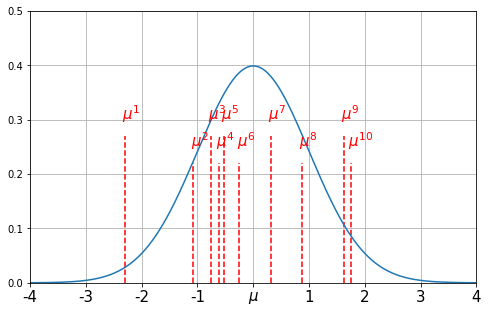
\includegraphics[width=0.7\textwidth]{figures/lesson4_33_0.png}
	\caption{Distribution of a series of ten Monte Carlo experiments around the \emph{true} value $\mu$.}
	\label{fig:repeated_MC}
\end{figure}

Therefore \( \hat{\mu}_n - \mu \) is approximately distributed as 
\[ \hat{\mu}_n - \mu \approx \frac{\sigma}{\sqrt{n}}Z \]
where $Z=\mathcal{N}(0, 1)$ is the standard Gaussian.

This means that given a Monte Carlo experiment the true value $\mu$ will lay in the interval $\hat{\mu}_n \pm  \frac{\sigma}{\sqrt{n}}Z$ around our best estimate. 
\begin{figure}[h]
	\centering
	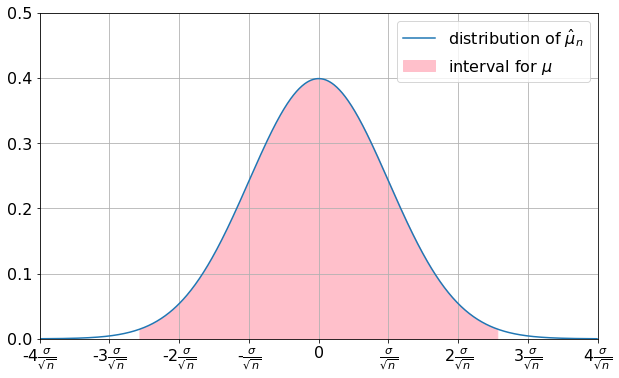
\includegraphics[width=0.7\textwidth]{figures/confidence_interval.png}
	\caption{Confidence interval graphical explanation.}
	\label{fig:confidence}
\end{figure}
Referring to Fig.~\ref{fig:confidence} we can write:
\[\mathbb{P}\Big(\hat{\mu}_n - \frac{1.96\sigma}{\sqrt{n}} \le \mu \le \hat{\mu}_n + \frac{1.96\sigma}{\sqrt{n}}\Big) = 0.95 \]
which corresponds to the shaded area.

The interval above is called 95\% \textbf{confidence interval}. If a variable $X$ is distributed as a Gaussian $\mathcal{N}(\mu, \sigma^2)$ then
\[\mathbb{P}(\mu - 1.96\sigma \le X \le \mu+ 1.96\sigma) = 0.95 \]
because the interval $\pm 1.96\sigma$ covers 95\% of the total area under the Gaussian, in formula $\Phi(1.96)=0.975$ where $\Phi$ is the Gaussian cumulative distribution function.

To construct a confidence interval with a confidence level $\alpha$ different from 0.95, we have to find a number $A$ such that
\begin{equation}
	\Phi(A) = 1 - \frac{1-\alpha}{2}\quad\implies\quad A = \Phi^{-1}\left(\cfrac{1+\alpha}{2}\right)
	\label{for:A}
\end{equation}
then the $\alpha$-confidence interval
\[\mathbb{P}(\mu - A\sigma \le X \le \mu+ A\sigma) = \alpha \]

The width of the confidence interval is a measure of the accuracy of our estimate.
$\alpha$-confidence interval can be expressed in terms of repeated
experiments like the following: if you repeat many time a simulation,
the fraction of calculated confidence intervals (which would differ for each sample) that contains
the true parameter would tend toward $\alpha \%$ (beware! anyway in $1-\alpha\%$ of cases it is outside the interval!).

Below an example of how to compute a confidence level in \texttt{python} given a set of fake simulations. To note that the inverse of the Gaussian CDF $\Phi^{-1}$, used in Equation~\ref{for:A}, is computed with the method \texttt{norm.ppf()} (more details on CDF in Chapter~\ref{quantile-function}).

\begin{tcolorbox}[breakable, size=fbox, boxrule=1pt, pad at break*=1mm,colback=cellbackground, colframe=cellborder]
\begin{Verbatim}[commandchars=\\\{\}]
\PY{k+kn}{import} \PY{n+nn}{numpy} \PY{k}{as} \PY{n+nn}{np}
\PY{k+kn}{from} \PY{n+nn}{scipy}\PY{n+nn}{.}\PY{n+nn}{stats} \PY{k}{import} \PY{n}{norm}
		
\PY{n}{samples} \PY{o}{=} \PY{p}{[}\PY{l+m+mf}{1.}\PY{p}{,}\PY{l+m+mf}{2.}\PY{p}{,}\PY{l+m+mf}{3.}\PY{p}{,}\PY{l+m+mf}{4.}\PY{p}{,}\PY{l+m+mf}{4.}\PY{p}{,}\PY{l+m+mf}{4.}\PY{p}{,}\PY{l+m+mf}{5.}\PY{p}{,}\PY{l+m+mf}{5.}\PY{p}{,}\PY{l+m+mf}{5.}\PY{p}{,}\PY{l+m+mf}{5.}\PY{p}{,}\PY{l+m+mf}{4.}\PY{p}{,}\PY{l+m+mf}{4.}\PY{p}{,}\PY{l+m+mf}{4.}\PY{p}{,}\PY{l+m+mf}{6.}\PY{p}{,}\PY{l+m+mf}{7.}\PY{p}{,}\PY{l+m+mf}{8.}\PY{p}{]}
\PY{n}{alpha} \PY{o}{=} \PY{l+m+mf}{0.95}
		
\PY{n}{X} \PY{o}{=} \PY{n}{np}\PY{o}{.}\PY{n}{array}\PY{p}{(}\PY{n}{samples}\PY{p}{)}
\PY{n}{A} \PY{o}{=} \PY{n}{norm}\PY{o}{.}\PY{n}{ppf}\PY{p}{(}\PY{p}{(}\PY{l+m+mi}{1} \PY{o}{+} \PY{n}{alpha}\PY{p}{)}\PY{o}{/}\PY{l+m+mi}{2}\PY{p}{)}
\PY{n}{m}\PY{p}{,} \PY{n}{se} \PY{o}{=} \PY{n}{np}\PY{o}{.}\PY{n}{mean}\PY{p}{(}\PY{n}{X}\PY{p}{)}\PY{p}{,} \PY{n}{np}\PY{o}{.}\PY{n}{std}\PY{p}{(}\PY{n}{X}\PY{p}{)}
\PY{n}{h} \PY{o}{=} \PY{n}{A}\PY{o}{*}\PY{n}{se}\PY{o}{/}\PY{n}{np}\PY{o}{.}\PY{n}{sqrt}\PY{p}{(}\PY{n+nb}{len}\PY{p}{(}\PY{n}{samples}\PY{p}{)}\PY{p}{)}
\PY{n+nb}{print} \PY{p}{(}\PY{l+s+s2}{\PYZdq{}}\PY{l+s+si}{\PYZob{}:.0f\PYZcb{}}\PY{l+s+si}{\PYZpc{} c}\PY{l+s+s2}{onfidence interval: }\PY{l+s+si}{\PYZob{}\PYZcb{}}\PY{l+s+s2}{ +\PYZhy{} }\PY{l+s+si}{\PYZob{}\PYZcb{}}\PY{l+s+s2}{\PYZdq{}}\PY{o}{.}\PY{n}{format}\PY{p}{(}\PY{n}{alpha}\PY{o}{*}\PY{l+m+mi}{100}\PY{p}{,} \PY{n}{m}\PY{p}{,} \PY{n}{h}\PY{p}{)}\PY{p}{)}
		
95\% confidence interval: 4.4375 +- 0.8119808363806419
\end{Verbatim}
\end{tcolorbox}

Using the confidence interval we can check whether the Monte Carlo estimate of the swaption payoff is in agreement with what computed using the Black-Scholes formula.
Let's then calculate the 95\% confidence level for the swaption simulation:

\begin{tcolorbox}[breakable, size=fbox, boxrule=1pt, pad at break*=1mm,colback=cellbackground, colframe=cellborder]
\begin{Verbatim}[commandchars=\\\{\}]
\PY{n}{npv\PYZus{}error} \PY{o}{=} \PY{l+m+mf}{1.96} \PY{o}{*} \PY{n}{np}\PY{o}{.}\PY{n}{std}\PY{p}{(}\PY{n}{discounted\PYZus{}payoffs}\PY{p}{)}\PY{o}{/}\PY{n}{sqrt}\PY{p}{(}\PY{n}{n\PYZus{}scenarios}\PY{p}{)}
				
\PY{n+nb}{print}\PY{p}{(}\PY{l+s+s2}{\PYZdq{}}\PY{l+s+s2}{Swaption NPV: }\PY{l+s+si}{\PYZob{}:.2f\PYZcb{}}\PY{l+s+s2}{ EUR (+/- }\PY{l+s+si}{\PYZob{}:.2f\PYZcb{}}\PY{l+s+s2}{ EUR with 95}\PY{l+s+si}{\PYZpc{} c}\PY{l+s+s2}{onfidence)}\PY{l+s+s2}{\PYZdq{}}\PYZbs{}
      \PY{o}{.}\PY{n}{format}\PY{p}{(}\PY{n}{npv\PYZus{}mc}\PY{p}{,} \PY{n}{npv\PYZus{}error}\PY{p}{)}\PY{p}{)}

Swaption NPV: 218833.40967569317 EUR (+/- 108.1575900210255 EUR with 95\% confidence)
\end{Verbatim}
\end{tcolorbox}

The NPV calculated via the Black-Scholes formula
falls well within the confidence interval produced by the Monte Carlo
simulation

\begin{itemize}
\tightlist
\item
  Swaption NPV (BS): \euro{218896}
\item
  Swaption NPV (MC): \euro{218833}
\end{itemize}
so we can assert that the two estimates are in agreement at the 95\% confidence level.
